%! suppress = MissingImport
In this section, you will install the ``slider'' switches that toggle between their two positions, holding their position until toggled again.
We will wire them such that when a switch is toggled to the left, it will produce a 0, and when it is toggled to the right, it will produce a 1.
Figure~\ref{fig:switch-diagram} shows a diagram of the wiring for the slider switches.

\begin{figure}[p]
    \centering
    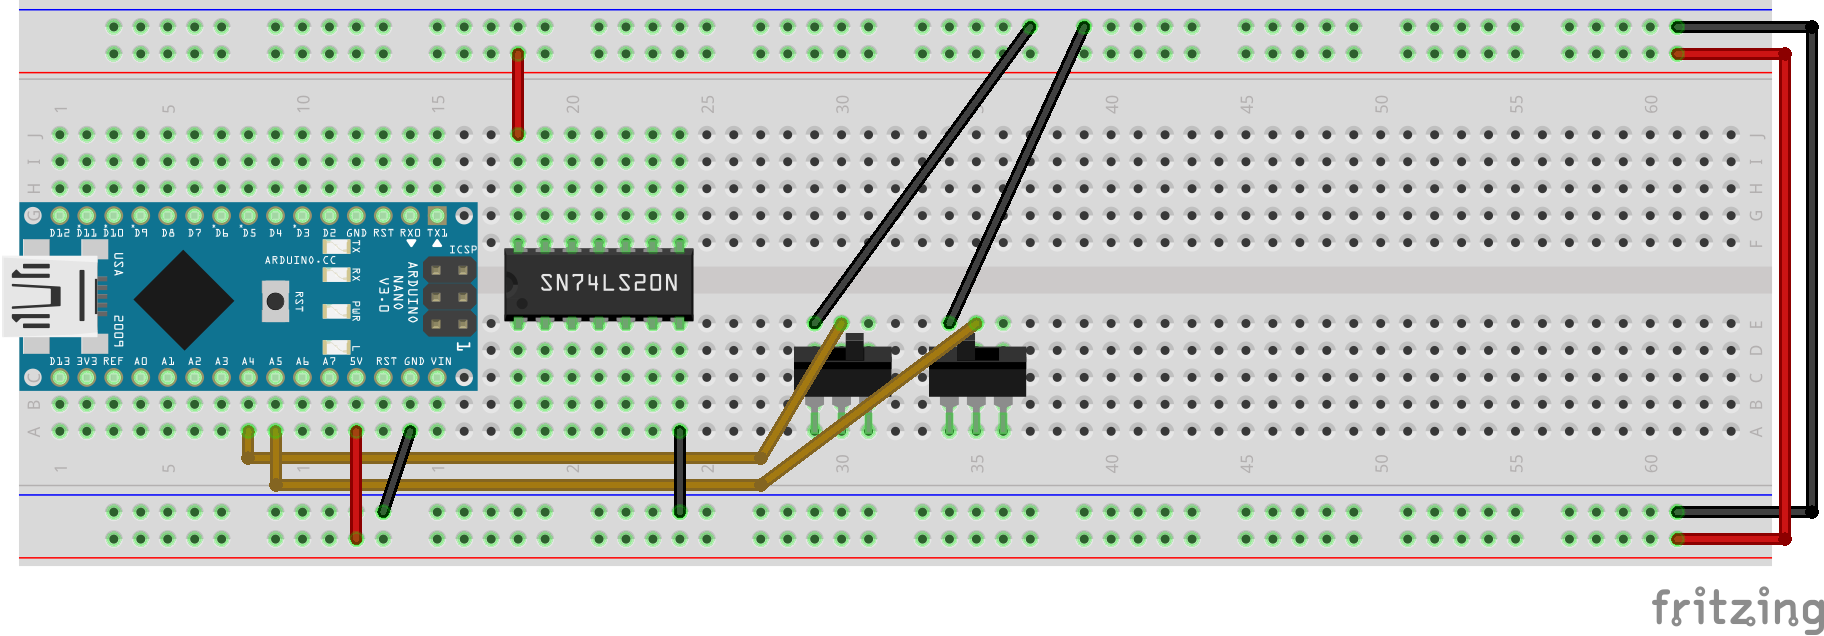
\includegraphics[width=0.9\textwidth]{fritzing_diagrams/switch-spi}
    \caption{Diagram of wiring associated with toggle switch input.
        \label{fig:switch-diagram}}
\end{figure}

\disconnect\

Insert one slider switch into contact points a29-a31.
Peel off one wire from the \rainbow, and use it to connect contact point e29 to the upper \ground.
Place the other slider switch into contact points a34-a36.
Peel off another wire from the \rainbow, and use it to connect contact point e34 to the upper \ground.
% See Figure~\ref{fig:switch-power-ground}.

Peel off one wire from the \rainbow, and use it to connect contact point d30 (electrically connected to the left switch's center pin) to contact point a8 (electrically connected to the \developmentboard's \texttt{A4} pin).
Peel off another wire from the \rainbow, and use it to connect contact point d35 (electrically connected to the right switch's center pin) to contact point a9 (electrically connected to the \developmentboard's \texttt{A5} pin).
% See Figure~\ref{fig:switch-nano}. See Figure~\ref{fig:switch-spst}.

The switches' right pins will not be electrically connected to anything.

% \begin{figure}
%     \centering
%     \subfloat[The slider switches, each with their left pin grounded and their
%         right pin connected to 5V.]{
%         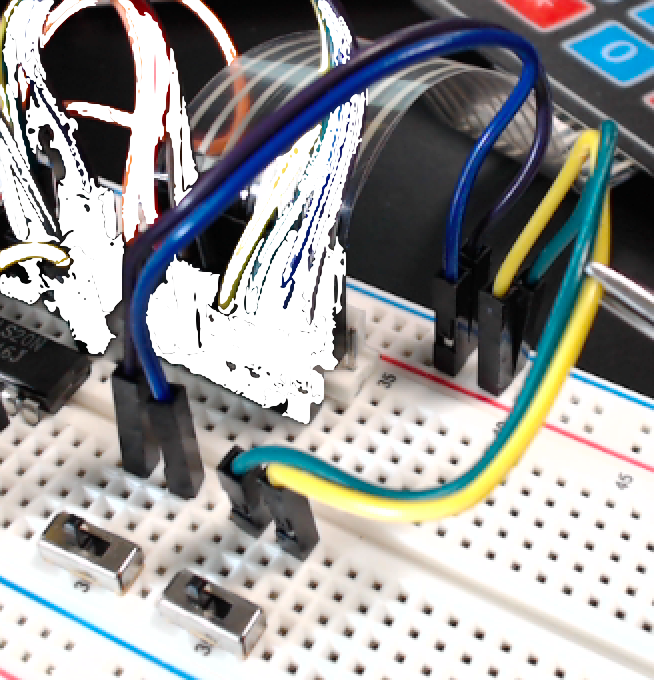
\includegraphics[width=0.3\textwidth]{switch-power-ground}
%         \label{fig:switch-power-ground}
%     }
%     \hfil
%     \subfloat[Connections between the \developmentboard\ and the slider switches.]{
%         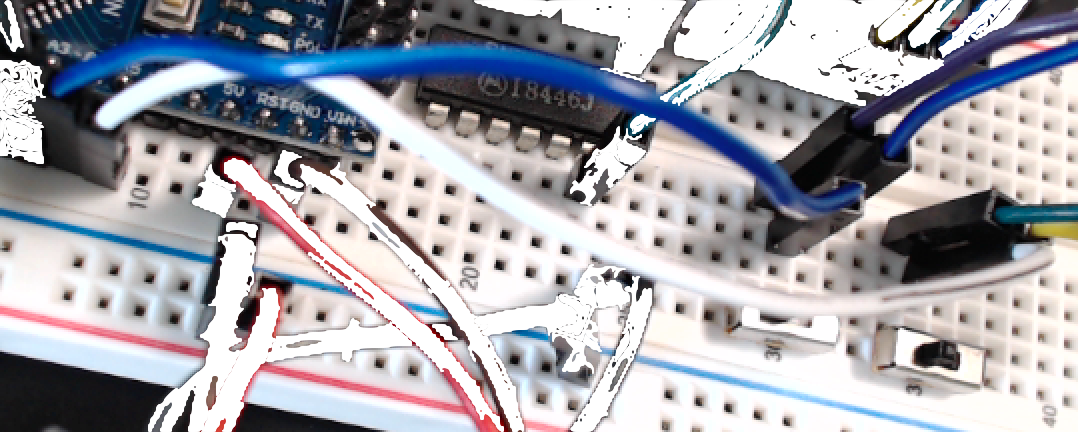
\includegraphics[width=0.6\textwidth]{switch-nano}
%         \label{fig:switch-nano}
%     }
%     \caption{Wiring the Slider Switches}
% \end{figure}

\begin{figure}
    \centering
    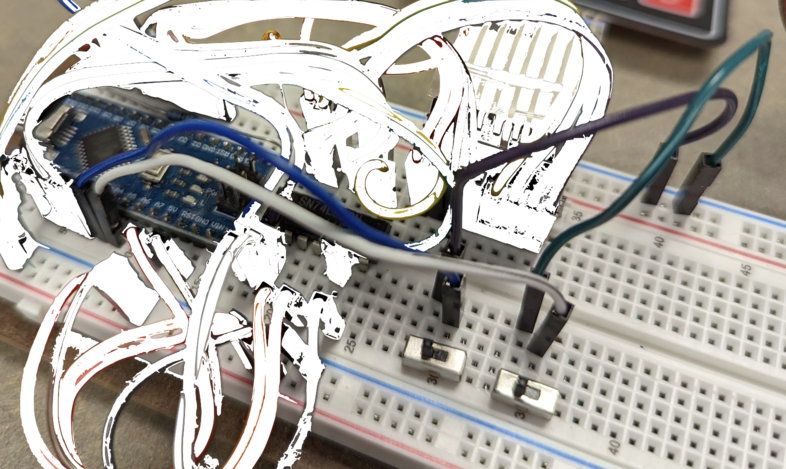
\includegraphics[width=0.6\textwidth]{direct/switches/switch-spst}
    \caption{The slider switches, each with one pin grounded, one pin connected to the \developmentboard, and one pin floating. \label{fig:switch-spst}}
\end{figure}

When you have finished setting up the switches' wiring, there should be the
electrical connections described in Table~\ref{tab:switch}.

\begin{table}
    \begin{center}\begin{tabular}{||c|c|c||} \hline\hline
    Switch                      & \developmentboard\ pin    & Pulled High/Low \\ \hline
    Left switch's left pin      &               & Pulled Low \\
    Left switch's center pin    & \texttt{A4}   & \\
    Left switch's right pin     & \multicolumn{2}{c||}{not connected / floating} \\
    Right switch's left pin     &               & Pulled Low \\
    Right switch's center pin   & \texttt{A5}   & \\
    Right switch's right pin    & \multicolumn{2}{c||}{not connected / floating} \\ \hline\hline
    \end{tabular}\end{center}
    \caption{Electrical Connections for Slider Switches.\label{tab:switch}}
\end{table}

\checkpoint{inserted and wired the slider switches}

Connect your \developmentboard\ to the computer.
In the IDE's Serial Monitor, notice that the LEFT~SWITCH is 0 when the left switch is toggled to the left, and it is 1 when the left switch is toggled to the right.
Similarly, the RIGHT~SWITCH's value is 0 or 1, depending on whether the right switch is toggled to the left or right.